\chapter{Analyse comparative des  performances}
Dans cette partie, nous analysons les résultats et performances des différentes méthodes et optimisations implémentées.

Pour cela, nous avons lancé des séries de tests avec 100 itérations et avec des nombres particules différents. Nous avons donc mesuré et sommé le temps concerné pour chaque itération afin d'effectuer une moyenne pour chaque nombre de particules.

\section{Construction de l'arbre}
\begin{center}
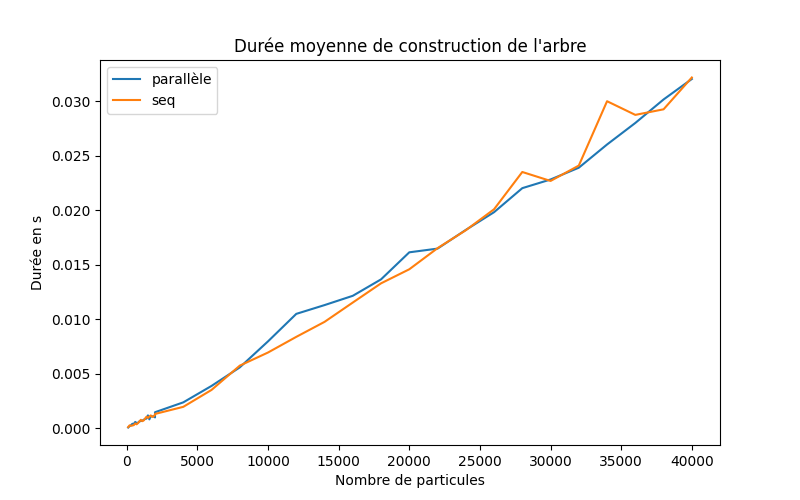
\includegraphics[scale=0.6]{./resultats/tree_comparison.png}
\captionof{figure}{Durée moyenne de construction de l'arbre}
\label{figbh}
\end{center}

On peut voir sur la figure que pour des plus petits nombres de particules, la version séquentielle aura légèrement de meilleure performance alors que pour des valeurs plus grandes(>250000), la version parallèle sera plus intéressante. Mais de manière globale, l'algorithme de création de l'arbre est aussi performant avec ou sans parallélisation. On peut alors penser que la parallélisation ne fonctionne pas correctement à cause de problème de compétition entre les threads : les insertions des particules ne sont pas totalement indépendantes.

\section{Comparaisons des méthodes}

\begin{minipage}[c]{.46\linewidth}
     \begin{center}
             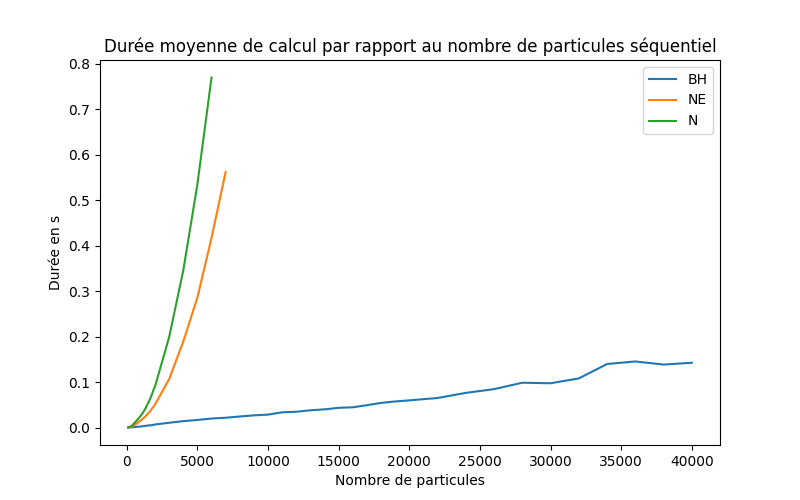
\includegraphics[width=9cm]{./resultats/method_comparison_seq.png}
         \end{center}
   \end{minipage} \hfill
   \begin{minipage}[c]{.46\linewidth}
    \begin{center}
            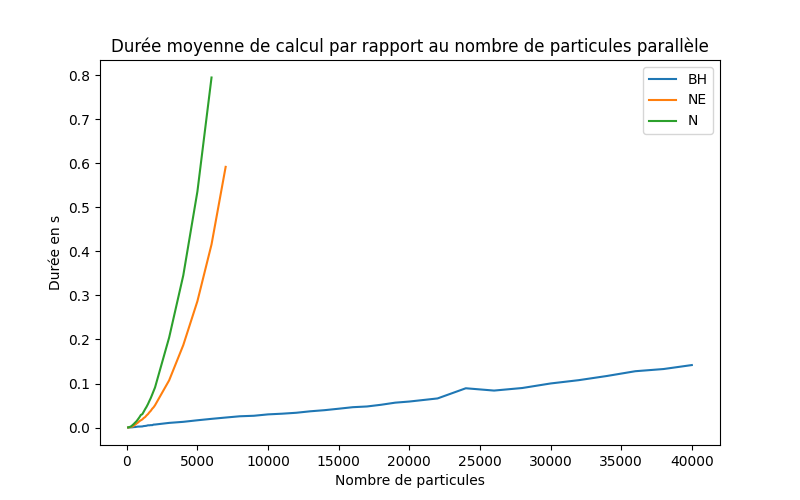
\includegraphics[width=9cm]{./resultats/method_comparison_par.png}
        \end{center}
 \end{minipage}
 
Les résultats confirment la théorie. Il est clair que les méthodes brutes ont une complexité en $O(N^2)$ alors que l'algorithme de Barnes-Hut a une complexité bien inférieure en $O(Nlog(N))$.
On peut également confirmer que l'algorithme naïf optimisé a une meilleure complexité que la version naïve.
 
\section{Séquentiel et parallèle}

\subsection{Algorithme de Barnes-Hut}
\begin{center}
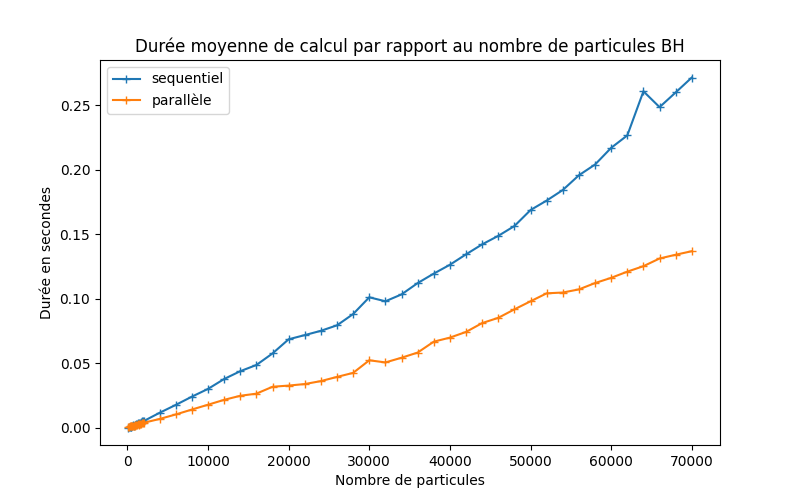
\includegraphics[scale=0.6]{./resultats/comparison_BH.png}
\captionof{figure}{Résultats pour l'algorithme de Barnes-Hut}
\label{figbh}
\end{center}

On peut voir sur la figure que globalement la parallélisation n'améliore pas énormément l'efficacité de l'algorithme. Cependant, malgré tout, la version parallèle a une complexité plus "stable" et pour un grand nombre de particules(>2000), il sera plus intéressant.

\subsection{Naïve optimisée}
\begin{center}
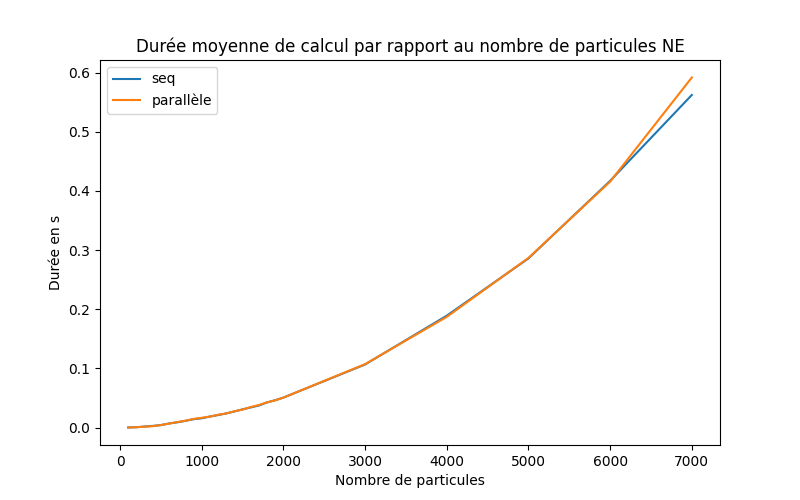
\includegraphics[scale=0.6]{./resultats/comparison_NE.png}
\captionof{figure}{Résultats pour l'algorithme naïf optimisé}
\label{figbh}
\end{center}

Les résultats montrent clairement que la parallélisation n'améliore pas la complexité de l'algorithme et que pour des grandes valeurs elle ralentit les calculs.
Cela s'explique simplement par les situations de compétition des threads lors de l'accès aux données. En effet, chaque calcul de force dépend de ceux des particules précédentes ce qui ralentit les calculs au final.

\subsection{Naïve}
\begin{center}
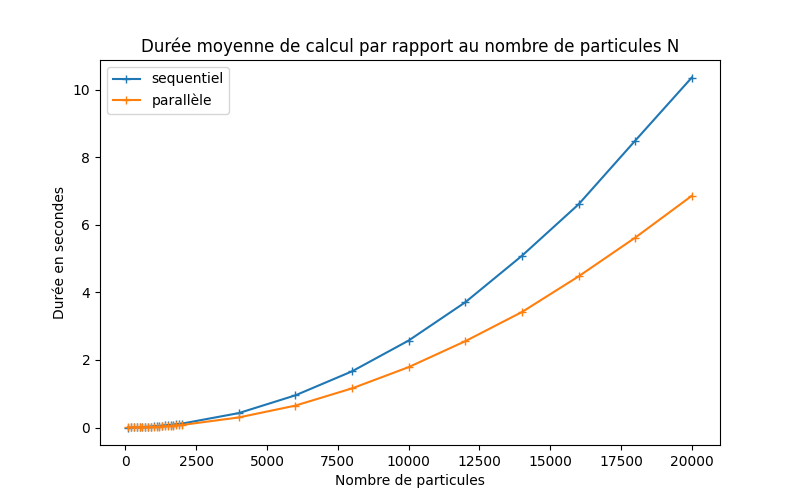
\includegraphics[scale=0.6]{./resultats/comparison_N.png}
\captionof{figure}{Résultats pour l'algorithme naïf }
\label{figbh}
\end{center}

De nouveau, la parallélisation ne change pas les performances de l'algorithme ce qui est plutôt surprenant étant donné que les calculs de forces sont tous indépendants les uns des autres.
Cependant, on pourrait expliquer cela par la répétitions des calculs pour chaque particules étant donné que l'on n'utilise pas le principe d'action-réaction.

\vspace{2mm}

Les résultats obtenus dans cette partie ont permis de vérifier les résultats théoriques par rapport aux performances des algorithme: l'algorithme de Barnes-Hut est bien plus performant que les autres. De plus, ils ont également montré que l'algorithme de Barnes-Hut est intéréssant à parallèliser alors que les autres ne subissent aucune augmentation de performance.